\documentclass[main]{subfiles}

\begin{document}

\jsv{Pour chacun des 4 assembleurs décrit, une vue schématique des étapes serait la bienvenue, voire les mettre tous sur une même figure avec des briques qui portent des même noms : OLC, minimizer, etc. Je ne sais pas du tout si c'est facilement réalisable.}

\chapter{Long reads assembly tools state of the art}\label{chapter:sota}

In this chapter we present some long-read assembly tools we select this tools because method and algorithm used in it was representative how other tools work in addition, these tools are recognized by the community for their quality. 


\jsv{Etoffer l'intro. Faire le lien avec les chapitres précédents et le chapitre suivant. Dire par exemple qu'une fois un ensemble de reads propres est disponible on peut alors réaliser l'assemblage. Redire en quoi consiste l'assemblage. Puis indiquer en quelques mots en quoi les longs reads ont nécessité de construire de nouveaux outils. C'est aussi le moment de citer Celera comme tu le fais. Ensuite, tu peux dire qu'il y a pléthore d'outils mais que tu te concentre sur certains. Tu les cites avec les numéros de section afin de donner le plan de lecture. Enfin tu termines avec l'objectif de cette description : montrer qu'on peut aller chercher/intervenir sur des phases intermédiaires, ce qui sera abordé dans le chapitre suivant.}

\section{A Pipeline with correction \canu} \label{section:sota:canu}

\jsv{Idem, ajouter un peu de liant, une phrase suffit. Canu \cite{canu} a été proposé en 20XX et est l'un des tout premier assembleur long read populaire capable de traiter des reads ONT et PacBio après HGAP (pour PacBio)}

\canu is based on \toolsname{Celera} \cite{celera_first, celera_second}, we can split the \canu pipeline in three step, correction, trimming and assembly, before each step \canu search overlap between reads.

\jsv{Juste avant tu indiques trois étapes, la première est correction, c'est troublant que le titre du premier paragraphe soit Overlapping. J'écrirai we can split the \canu pipeline in three steps, correction, trimming and assembly decribed below. Nevertheless, before each of these steps \canu search overlap between reads. We thus start by explaining how overlaps are computed.}

\paragraph{Overlapping}

\jsv{Commencer par dire que les overlaps sont calculés avec MHAP}

To avoid all versus all alignment \mhap try to estimate which read share a common part by estimate a Jaccard distance between the set of \kmers of two reads. The Jaccard distance, present in equation \ref{sota:equ:jaccard_dist} evaluate the distance between two set by divide the intersection of set by union of set.

\begin{equation}
J_{\delta}(A,B) = 1 - J(A,B) = 1 -  J(A,B) = 1 - \frac{|A \cap B|}{|A \cup B|}
\label{sota:equ:jaccard_dist}
\end{equation}

Enumerate all \kmers of each reads and compute intersection and union of each set take many times. \mhap select a subset of \kmers to represent the read and compute a mash distance \cite{mash_distance} see equation \ref{sota:equ:mash_dist_def} 

\begin{equation}
J(A,B) = \frac{|A \cap B|}{|A \cup B|} \approx \frac{|S(A \cup B) \cap S(A) \cap S(B)|}{|S(A \cup B)|}
\label{sota:equ:mash_dist_def}
\end{equation}

$S(A)$ is a \kmers set compose by $s$ first \kmers of set $A$. \citeauthor{mash_distance} evaluate the error between mash distance and Jaccard distance was in $\mathcal{O}(\frac{1}{\sqrt{s}})$, by default in \mhap $s=512$ so the error was smaller than 0.05.

In \mhap order \kmer with a \texttt{tf-idf} score, see equation \ref{sota:equ:tf_idf_def}. The \texttt{tf-idf} score come for text search domain. \texttt{tf-idf} evaluate if this term is specific to this document. \texttt{tf} for term frequency indicate if the term was present many times in document, $n_{i,j}$ how many time the term $i$ was present in document $j$ divide by the number of term in document $j$. \texttt{idf} for inverse document frequency evaluate if the term was present in many document or just in some document, $|\mathcal{D}|$ the number of document in dataset divide by $|\{d_{j}:t_{i}\in d_{j}\}|$ the number of document where the term $i$ was present.

\begin{equation}
\mathrm{tf-idf_{i,j}} = \mathrm{tf_{i,j}} \cdot \mathrm{idf_{i}} = \frac{n_{i,j}}{\sum_{k}n_{k,j}} \cdot \log{\frac  {|\mathcal{D}|}{|\{d_{j}:t_{i}\in d_{j}\}|}}
\label{sota:equ:tf_idf_def}
\end{equation}

In \mhap term was \kmer and document was read, this technique permit to reduce the number of \kmer in set and keep \kmer specific to a read. If two read share specific \kmer they probably share a common part.

If two reads have a small mash distance \mhap compare the position of each \kmer in reads to determinate the overlap position.

The size of \kmer was very important to if k is too large many \kmer contains error the size of intersection was reduce and \mhap can miss overlap. Moreover size of sketch have a huge impact if it's to small the read was sub-sample if it's to large compute mash distance take more time, but with long-reads dataset the length of reads can be very different choose a good sketch size for this type of data isn't easy.

\jsv{Très bien la critique. Mais on s'attend à une conclusion sur comment cela fonctionne en pratique.}

\paragraph{Correction}

In \canu correction was performed by a part of \toolsname{FALCON} \cite{falcon}, \toolsname{falcon\_sense}. \jsv{On en déduit que FALCON précède Canu, ce serait bien de dire en un mot pourquoi tu ne décris pas FALCON} In this section we didn't present in details how \toolsname{falcon\_sense} work but only the main idea.

Some correction tools as \toolsname{falcon\_sense} use a Partial Order Alignment (POA) (introduce in \cite{poa}) to perform long read correction. For each read \texttt{$R_1$} we recruit all read share an overlap with him, and perform an exact alignment with him. This alignment was use to build a POA graph, in POA graph each base was a node and a direct edge was create between two base if the first base was before the second one in an alignment. If an edge was present in two alignment her weight was increment. After all alignment was add in the POA graph, we search weighed path in this graph, and follow to reconstruct the corrected sequence. An example of POA graph construction was present in figure \ref{sota:fig:canu:correction}

\begin{figure}[ht]
    \centering
    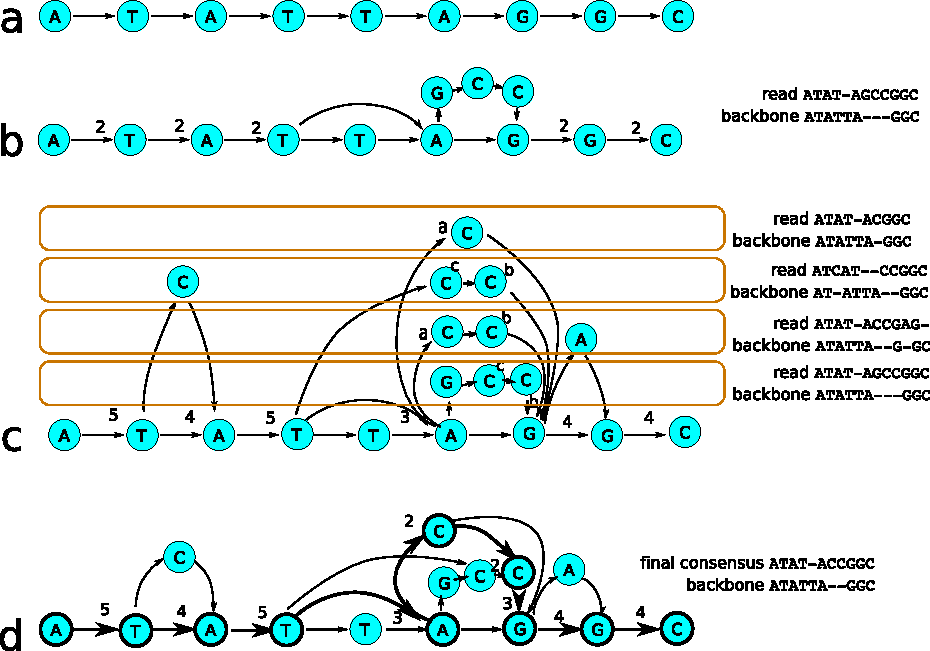
\includegraphics[width=\textwidth]{state_of_the_art/images/POA_explain.pdf}
    \caption{Sequence need to be correct was represent as a graph, each base was a node and if a base is follow by another an directed edge was build. (b) was the representation of sequence \texttt{ATATTAGGC} (call backbone in this figure), (b) We add the result of alignment of one read in the graph, number upper than edge was her weigth if and edge exist in some 3 alignment her weight was egal to 3, (c) We add all other alignment in the graph, (d) the bold path was choose a the correct path because it was supported by more alignment. This figure was originaly present in Supplementary material of \hgap \cite{hgap}}
    \label{sota:fig:canu:correction}
\end{figure}

\paragraph{Trimming}

The trimming step will remove the parts of the reads that are not supported by the other reads, see Figure \ref{sota:fig:canu:trimming}. For each reads we will analyze its coverage curve and remove the parts of the reads that are not sufficiently covered, for trimming \canu use an homemade tools. 
\jsv{on aimerait savoir quelle est la couverture minimale par défaut}

\begin{figure}[ht]
    \centering
    \subfile{state_of_the_art/tikz/trimming.tex}
    \caption{Black line was a reads, the \canu trimming step keep only the blue part of read $R_0$, part covered by other read.}
    \label{sota:fig:canu:trimming}
\end{figure}

\paragraph{Assembly}

\canu assembly step is based on \OLC paradigm \jsv{faire un renvoi à l'introduction où tu décris le paradigme OLC}, with some specificity. \canu build a Best Overlap Graph (BOG) for each not contained read only two overlap are kept in the graph, the best overlap for each read extremity, in \canu the best overlap was the longest overlap. After this graph construction step performed, some clean step was run, remove tips and little buble \jsv{faire référence à la définition dans l'introduction}.

This BOG was used as a scaffold to generate assembly, by remapping read against this scaffold, \canu try to detect repetition, larger than read not show in BOG as loop, and to call read to build a consensus after. Each simple path in BOG was used to build a contig. 

By remapping reads on the BOG \canu can build a consensus and detect repetition didn't observe in graph. BOG was an aggressive strategy to avoid transitive edge and reduce graph size but they can mask an edge denote a repetition this check was required to. 
\jsv{une illustration schématique serait bienvenue}


\section{Pipeline without correction \miniasm} \label{section:sota:miniasm}

\minimap and \miniasm was an assembly pipeline proposed in \cite{miniasm_minimap} and \cite{minimap2}, the main purpose of this pipeline is to demonstrate we can perform a long read assembly without correct long read before.

\jsv{Il faudrait comme pour Canu indiquer les étapes, c'est le moment de dire que la stratégie est un peu différente : filtre vs correction+trimming, au lieu de le dire plus loin.}

\subsection{\minimap}

Main idea to \minimap (similar to \mhap) is we can represent a read as a set of some minimal kmer, and if two read share same succession of minimal kmer we can suppose this two read share an overlap.

A minimal kmer is a the kmer for a set of consecutive kmer than minimize her score, the score function was the same during all analyse and for the same set of consecutive kmer the same kmer was the minimizer. Moreover a kmer can be minimizer of some consecutive set of kmer, if no other kmer with lowest score come in window. 

\begin{figure}[ht]
    \centering
    \subfile{state_of_the_art/tikz/minimizer.tex}
    \caption{The red kmer was the minimizer of the read box and the blue kmer was the minimizer of the blue box. \textcolor{red}{JSV: because \dots}}
    \label{sota:fig:miniasm:minimizer}
\end{figure}

The minimal \kmer can represent many other read, this technique can be compare to a loosly compression. \jsv{je ne comprends pas, compression avec ou sans perte}

\minimap build an index where each minimizer are associate to reads where minimizer is present and position of this minimizer in reads.

With this index \minimap can collect position of similar minimizer between two reads, with this collection of position \minimap search the largest co-linear match, a succession of similar minimizer in each reads with coherent position, same order of minimizer and similar distance between each minimizer. Figure \ref{sota:fig:miniasm:mapping} show an overview of a overlap of two reads in \minimap.

\begin{figure}[ht]
    \centering
    \subfile{state_of_the_art/tikz/minimap.tex}
    \caption{$Read_A$ and $Read_B$ was represent by black arrow. Common minimizer of $Read_A$ and $Read_B$ was represent by blue and red arrow respectively. Green arrow was a co-linear chain, purple arrow was another co-linear chain, black arrow didn't participate to a co-linear chain. \textcolor{red}{JSV: conclusion ?}}
    \label{sota:fig:miniasm:mapping}
\end{figure}

\minimap report overlap where the number of match is sufficient (upper than a threshold) and  total length of putative overlap was sufficient. 

\subsection{\miniasm}

\miniasm didn't perform correction but they didn't take all information from reads and overlap, some filtering operation was performed.

For each read \miniasm perform coverage analysis of reads based on mappings identify by \minimap, by default only the longest part of reads with a coverage upper than three are kept. \minimap report for each read, read length, position of first and last kmer, number of bases in kmer exact match,  and a mapping quality and some option field in SAM like format can be present too.

\begin{figure}[ht]
    \centering
    \subfile{state_of_the_art/tikz/miniasm_overlap.tex}
    \caption{\miniasm classify overlap in three type of dovetail, internal match and containment overlap. Black grey region correspond to part of read between first and last minimizer. Light grey region was called overhang region, it's out of minimizer range. If overhang was large compare to overlap region we can supects this overlap isn't a true overlap.}
    \label{sota:fig:miniasm:ovl_classification}
\end{figure}

Each overlap was classified, in three category:\jsv{expliquer pourquoi cette categorisation : in order to \dots}
\begin{itemize}
    \item internal match, this type of overlap probably correspond to a repetition smaller than reads length
    \item containment, a read of this overlap was contains in the other read it's same sequence
    \item dovetails, it's a end-to-end overlap
\end{itemize}
Figure \ref{sota:fig:miniasm:ovl_classification} show some exemple of this overlap. Containment read was removed, only dovetail overlap was used to build overlap graph. Tips, small bubble and transitive edge was removed after this step \miniasm take each simple path and concatenate substring of read between begins and the first position of overlap.

\miniasm was design to work on uncorrected read and didn't perform a consensus step so contigs generate by \miniasm contains many error and can't be used directly. We can run \minimap \miniasm pipeline with corrected read and a polishing tools on contig generate by \miniasm. 

\jsv{ajouter du liant : Very recently, another assembly tool,}
\toolsname{Ra}\cite{Ra} was a tools create to replace \miniasm in \minimap \miniasm pipeline. \toolsname{Ra} use an analysis of coverage curve of each reads to trimm not supported region, detect chimera and repeat region. Overlap on region marked as repeat are marked in string graph and not trusted. \toolsname{Ra} perform a real consensus step and run many polishing step with \toolsname{Racon}. \jsv{ajouter une analyse critique, même si cela ne fait que reprendre les conclusions de l'article parce que tu n'as pas toi-même de recul vu la publication récente : According to the authors, Ra performs \dots}

\section{\DBG like long reads assembly approach} \label{section:sota:wtdbg}

\jsv{je sais que je suis embêtant avec cela, mais ajoute du liant, dans l'intro du chapitre tu pourrais mentionner le fait que les approches DBG sont plutôt dévolues aux short read mais qu'on verra section X que celle-ci peut aussi être mise en oeuvre sur les long reads. Et ici  tu peux rappeler que cela a été utilisé avec succès en citant des outils et comme tu le fais ci-dessous dire pourquoi a priori ce n'est pas une méthode de choix }

The \DBG approach was not the preferred one for the assembly of long reads because :
\begin{itemize}
    \item reads contain a high error rate and therefore found error-free kmers was hard, this error can lead to expand size of graph and or mis-connection between part of graph.
    \item size of kmer was generaly lower than 100 base and manage larger kmer was hard without usage of many memory, moreover \DBG can't manage repetition larger kmer.
\end{itemize}

If we use \DBG naively for long read assembly, we can mis the main advantage of long-reads her length.

Some \flye and \wtdbg use \DBG approach with some modification to adapt this idea to long-read assembly.

\jsv{ici tu peux faire un peu de teasing en expliquant en deux mots ce qui rend l'approche adéquat y compris pour les long reads, cela montre que tu as du recul. Il me semble important de dire d'emblée que ce ne sont pas des DBG au sens strict.}

\subsection{\flye}

\flye\cite{Flye} was based on \abruijn\cite{abruijn} assembly tools. \abruijn didn't use a \DBG but a similar concept a \abreviation{ABG} (for A-Bruijn Graphs), in place of use a set of kmers as node \abreviation{ABG} use a set of chosen kmers, in place of build an edge between each kmer they share a k-1 overlap they build an edge with a weight equal to the distance of kmer in the original string between without create transitive edge.

To build the chosen \kmers set, \abruijn select kmers present many times in dataset this kmers was called in many tools \textit{solid} \kmers \jsv{citer le papier qui introduit la notion de solid kmer}. The more a \kmers is present in the dataset, the more sure you may be that this \kmers does not contain a sequencing error, if the genome coverage is 40x we can hope see \kmer, not include in a repetition, 40 times. Because when we sequence at 40x we didn't really read each base 40 times and when a sequence error appear we lost an occurrence of the kmers where this base was present, choose the number of times a kmer need to be present in dataset to be \textit{solid} was an hard task.

This modification help to clean sequencing error, but reduce the set of kmer fragment \DBG graphes it's why \abreviation{ABG} create edge not only when kmers share k-1 overlap. 

During the \abreviation{ABG} construction \abruijn store wich read generate wich graph path, this structure was usefull to found speedly overlap between reads. To build contigs \abruijn take a read $R_1$ found all overlap with help of \abreviation{ABG} if this local overlap graph didn't denote a fork, we have one read without successor and all reads have path in graph to this read, \abruijn extend the contig.

\abruijn can be roughly resume as mix of all assembly strategy, use \DBG to found overlap between read, build contigs by extension like \textit{greedy} methode but use \OLC to check they aren't integrate a repetition and a potential missassembly in contigs.

\flye was build on top of \abruijn, after \abruijn assembly \flye search self alignment in assembly. If extremity of contig are similar they are tag as repetition. \flye build a repetition graph, where repetition extremity as node and a edge was build when to repetition extremity was link in a contig. \flye use coverage information to take a clue on contig succession over untangle repetition. By analysis the topology of repetition graph \flye like \hinge can found a uniq traversal path to explain all repetition and found the genomic order of contig.

\jsv{citer hinge. hinge n'est pas décrit, sauf dans le papier, y faire référence. D'autre part est-ce le même graphe de répétitions ? Sinon, il est inutile de citer hinge ici.}

\subsection{\wtdbg}

\wtdbg \jsv{citer} use a \DBG approch to solve long-read assembly, isn't realy a \DBG but a "Fuzzy-Brujin graph" (\abreviation{FDBG}) \jsv{préciser si la notion est définie pour la première fois dans wtdbg}. To build this graph \wtdbg split read in bin with a fixed size (256 base pairs) and they store kmer present in each bin in a hash table.
To find overlap between reads wtdg2 use an hash table to compare the kmer composition between each reads and perform an exact alignment between each bin of reads. 

After this alignment step \wtdbg keep only in memory wich bin are align to which bin, and they build a k-bins each k-bins is a sequence of k successive bin in a read, \wtdbg can infer if two k-bins overlap if some bin in this two k-bins share an ovelap.

A group of k-bins are a node of \abreviation{FDBG}, \wtdbg build an edge between two node if a k-bins in each node are succesive in a read, after some cleanning step (pops bubbles, tips cleanning) \wtdbg build a consensus sequence with each simple path in \abreviation{FDBG}.

\section{New long read assembly}

\jsv{par New tu entends très récents}

\jsv{A nouveau une petit phrase d'intro ne ferait pas de mal}

\subsection{Peregrine}

\newcommand{\shimmer}{\toolsname{SHIMMER}}

\peregrine \cite{Peregrine} use \shimmer overlapper. \shimmer extend idea of minimizer \jsv{ajouter un rappel à minimap, cela fait du lien entre tes sections : defined in minimap}, we can have a minimizer of minimizer. \jsv{je dirais plutôt, la nouveauté c'est d'itérer le processus de construction de minimizer, avec pour objectif de XXX}
The layer-0 of minimizer was a basic minmizer process, like \minimap. After this step \shimmer, select minimizer they participate to the layer-1, they use a reduction factor, for a reduction factor $x$, $x$ minimizer was represent by the minimal minimizer of this set, this process can be repeat with many layer. When they choose the minimizer of $layer_n$ minimizer of $layer_{n-1}$ \shimmer take care of distance between each $layer_n$ minimizer to be shure they represent a distinct part of the read. \jsv{à ce point on a envie d'une indication sur le nombre de couches utilisées en pratique : reprendre un chiffre de l'article}

After this indexing step, \shimmer group reads they share many minimizer of last layer and perform a classic alignment to confirm overlap between reads. After this step \peregrine run a classic \OLC strategy to perform assembly.

\shimmer overlapping tools can be use to perform a mapping of read against contig or genome, after this remapping a poolshing step was perform, without a take an account to heterozygotie.

\peregrine was actually test only Circular Consensus (CCS) Pacbio data. Reads was sequence multiple time and a consensus was perform on all this sequencing, this technique reduce length of read but reduce the error level of sequencing too. Found overlap between reads with less error was easier and faster. This methode create by \peregrine tools was very interesting \jsv{tu apportes un jugement de valeur, il fat argumenter : pourquoi penses-tu que c'est intéressant, quel verrou cela permet-il de lever ?}, but they need to be validate on other type of data before they are generalize.

\subsection{Shasta}

\newcommand{\shasta}{\toolsname{Shasta}}

\shasta\footnote{https://github.com/chanzuckerberg/shasta/} isn't yet publish but the documentation present a huge overview of algorithm and method use by this assembly tools.

\jsv{j'inverserais les deux phrases, d'abord dire que c'est une approche par compression sans perte, puis dire comment c'est fait}
\shasta use read-length representation of reads, read-length representation was a loss-less compression method for text was contains a large repetition of same character. For example sequence \texttt{ACCTTTGAA}, was represent by two string $Sb$ \texttt{A C T G A} and $St$ \texttt{1 2 3 1 2}. To reconstruct original sequence we repeat $St_i$ time the $Sb_i$ letre.

This representation was interesting for long-reads data, because DNA contains sometimes same character repetition (called an homopolymer) and long-reads make many times error in homopolymer, read-length representation by squashing this region can avoid this type of error, and facilitate alignment of long-reads.

To perform read overlapping \shasta, didn't use a minimizer approach but something very close, the $Sb$ string of read was split in kmer and some kmer was selected randomly, and called marker, the set of marker was the same for all data set. Reads was now represent by a succession of marker it's a destructive compression. \jsv{je ne comprends pas, desctuctive or lossless ?}
Before search a colinear match of marker, to select reads with higher probability of match \shasta compute a modification of MiniHash Jaccard estimation \jsv{(see section XXX)} to avoid bias create by difference of length between reads.

To perform assembly \shasta create a marker graph, it's something similar to \DBG, where kmer was marker and an edge was build between two marker if a read contains this succession of marker, each edge was weighted by the number of reads they contains this succession, after a cleaning step of marker graph (removing transitive edge, tips and bubble) path in marker graph was select and reads participate to building of edge of this path was used to build a consensus sequence of contigs.

\shasta isn't yet publish they contains mainy interesting idea and author's plan some improvement for heterozygotie detection, resolution and performance improvement.

\section{Conclusion}


Long read assembly was an active field of search many tools was create each year, and long read and long read assembly tools was used to improve genome and build draft genome.
\jsv{il est nécessaire ici de synthétiser les idées des différents algos avant de dire qu'il reste des choses à faire}
But some challenge need to be address, many assembly step have important cost in computation time and memory usage \jsv{c'est justement une remarque que je e me faisais en lisant, à aucun moment tu ne discutes du temps pris pour assembler un génome ou bien de la mémoire nécessaire, que ce soit du temps/mémoire réel ou de la complexité algo, je pense crucial que tu abordes cette question, avec plus de détails que tu ne le fais dans la phrase suivante}. For exemple get an overlap search with high precision and recall and without excessive cost in computation time and memory usage. \cite{bench_ovl}.

The only one assembly they try to take in account heterozygotie was \toolsname{FALCON}, and in future \shasta, make difference between an sequencing error and a natural variant or heterozygotie. Get heterozygotie and variant phased or genome graph after assembly was interesting. But tools to extract all this information from read didn't exist yet

\jsv{si tu conclues ton chapitre comme cela alors le lecteur pense que les chapitres suivants vont essayer de présenter des méthodes plus efficaces et de traiter de l'hétérozygtie, ce qui n'est pas tout à fait le cas. Je pense qu'il faut terminer avec ton point de vue concernant de nouvelles méthodes : pas nécessaire obligatoirement de créer de nouvelles choses mais aller vers du raffinement de résultats existants. Appuyer sur l'importance de la prise en compte des "bons" overlap pour assembler.}


\onlyinsubfile{
\bibliographystyle{plainnat}
\bibliography{main}
\addcontentsline{toc}{chapter}{Bibliography}
}

\end{document}